\hyphenation{se-para-tion}
\hyphenation{theo-re-ti-cal}
\hyphenation{handed-ness}

%______________________ cp phase ______________________
\section{CP-mixing in \tH processes}\label{sec:cp}

In addition to the sensitivity to sign of the H-t coupling, the \tHq and \tHW processes have been proposed as a tool to investigate the possibility of a H-t coupling that does not conserve CP\cite{maltoni2,demartin,ellis}. %Current experimental results are consistent with SM H-V and H-t couplings; however, negative H-t coupling is not excluded completely \cite{comb_ht_couplings}.\\

In this thesis, the sensitivity of \tH processes to CP-mixing is also studied on the basis of References \cite{maltoni2,demartin} using the effective field theory framework where a generic particle ($X_0$) of spin-0 and a general CP violating interaction with the top quark (Htt coupling), can couple to scalar and pseudo-scalar fermionic densities. The H-W interaction is assumed to be SM-like. The Lagrangian modeling the H-t interaction is given by

\beqn
\Lagr_0^t = -\bar\psi_t\left(c_{\alpha}\kappa_{Htt}g_{Htt}+i s_{\alpha}\kappa_{Att}g_{Att}\gamma_5 \right)\psi_t X_0,
\label{eq:l_cp}
\eeqn

\noindent where $\alpha$ is the CP-mixing phase, $c_\alpha\equiv\cos\alpha$ and $s_\alpha\equiv\sin\alpha$, $\kappa_{Htt}$ and $\kappa_{Att}$ are real dimensionless re-scaling parameters\footnote{analog to $\kappa_t$ and $\kappa_V$} used to parametrize the magnitude of the CP-violating and CP-conserving parts of the amplitude. The model defines $g_{Htt}=g_{Att}=m_t/v=y_t/\sqrt{2}$ with $v\sim 246$ GeV the Higgs vacuum expectation value. In this parametrization, three special cases can be recovered

\begin{itemize}
\item CP-even coupling $\to \alpha=0^o$  
\item CP-odd coupling $\to \alpha=90^o$
\item SM coupling $\to \alpha=0^o$ and $\kappa_{Htt}=1$  
\end{itemize}

The loop induced $X_0$ coupling to gluons can also be described in terms of the parametrization above, according to

\beqn
\Lagr_0^{g} = -\frac{1}{4}\left(c_{\alpha}\kappa_{Hgg}g_{Hgg}G_{\mu\nu}^aG^{a,\mu\nu}+s_{\alpha}\kappa_{Agg}g_{Agg}G_{\mu\nu}^a\widetilde G^{a,\mu\nu} \right)X_0.
\label{eq:l_Hglu}
\eeqn

\noindent where $g_{Hgg}=-\alpha_s/3\pi v$ and $g_{Agg}= \alpha_s/2\pi v$ and $G_{\mu\nu}$ is the gluon field strength tensors. Under the assumption that the top quark dominates the gluon-fusion process at LHC energies, $\kappa_{Hgg} \to \kappa_{Htt}$ and  $\kappa_{Agg} \to \kappa_{Att}$, so that the ratio between the gluon-gluon fusion cross section for $X_0$ and for the SM Higgs prediction can be written as     

\beqn
\frac{\sigma_{NLO}^{gg \to X_0} }{\sigma_{NLO,SM}^{gg \to H}}=  c^2_\alpha\kappa^2_{Htt}+s^2_\alpha \left( \kappa_{Att}\frac{g_{ Agg}}{g_{Hgg}} \right)^2.
\label{eq:GFrate}
\eeqn

If the re-scaling parameters are set to

\beqn
\kappa_{Htt}=1, \qquad \kappa_{Att}= \left|\frac{g_{Hgg}}{g_{Agg}}\right|=\frac{2}{3}.
\eeqn

\noindent the gluon-fusion SM cross section is reproduced for every value of the CP-mixing angle $\alpha$; therefore, by imposing that condition to the Lagrangian density \ref{eq:l_cp}, the CP-mixing angle is not constrained by current data. Figure \ref{xsec_alpha_thq} shows the NLO cross sections for t-channel $tX_0$(blue) and $t\bar{t}X_0$ (red) associated production processes as a function of the CP-mixing angle $\alpha$. $X_0$ is a generic spin-0 particle with top quark CP-violating coupling. Re-scaling factors $\kappa_{Htt}$ and  $\kappa_{Att}$ have been set to reproduce the SM gluon-fusion cross sections.   

\begin{figure}[h!]
\centering
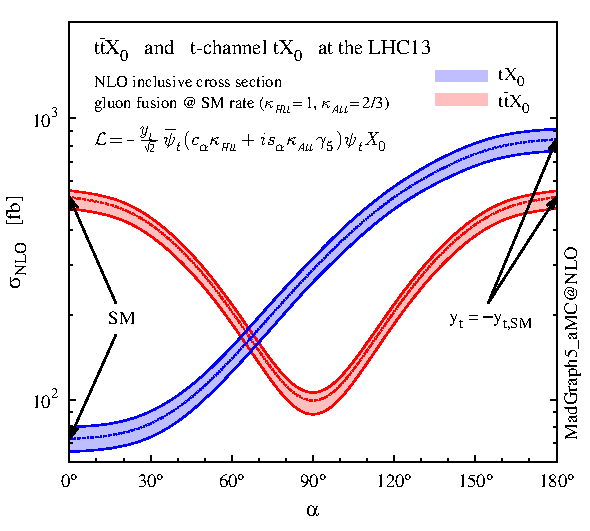
\includegraphics[scale=1.2]{xsec_alpha_thq}
\caption[NLO cross section for $tX_0$ and $t\bar{t}X_0$.]{NLO cross sections for t-channel $tX_0$(blue) and $t\bar{t}X_0$ (red) associated production processes as a function of the CP-mixing angle $\alpha$. $X_0$ is a generic spin-0 particle with top quark CP-violating coupling \cite{maltoni2}.} 
\label{xsec_alpha_thq}
\end{figure}

It is interesting to notice that the $tX_0$ cross section is enhanced, by a factor of about 10, when a continuous rotation in the scalar-pseudoscalar plane is applied; this enhancement is similar to the enhancement produced when the H-t coupling is flipped in sign with respect to the SM ($y_t=-y_{t,SM}$ in the plot), as showed in Section \ref{sec:thq}. In contrast, the degeneracy in the $t\bar{t}X_0$ cross section is still present given that it depends quadratically on the H-t coupling, but more interesting is to notice that $t\bar{t}X_0$ cross section is exceeded by $tX_0$ cross section after $\alpha\sim 60^o$.
\begin{figure}[h!]
\centering
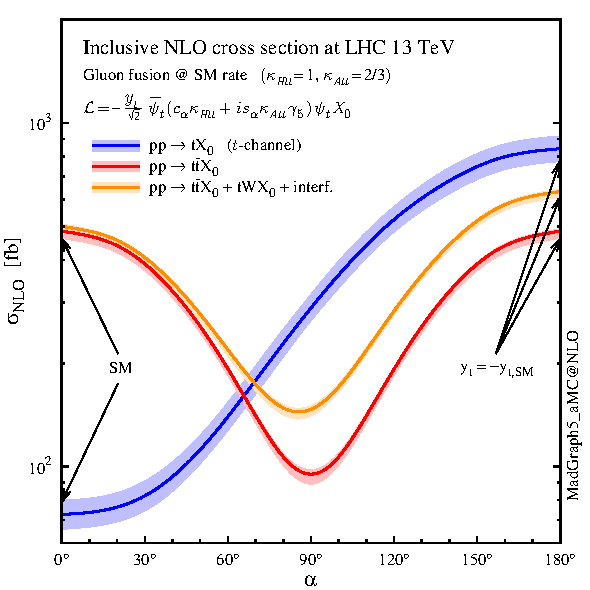
\includegraphics[scale=1.1]{xsec_alpha_thw}
\caption[NLO cross section for $tWX_0$, $t\bar{t}X_0$.]{NLO cross sections for t-channel $tX_0$(blue), $t\bar{t}X_0$ (red) associated production processes and combined $tWX_0 + t\bar{t}X_0$ (including interference) production as a function of the CP-mixing angle $\alpha$\cite{maltoni2}.} 
\label{xsec_alpha_thw}
\end{figure}

A similar parametrization can be used to investigate the \tHW process sensitivity to CP-violating H-t coupling. As said in \ref{sec:thq}, the interference in the W-associated channel is more complicated because there are more than two contributions and also there is interference with the \ttH production process.

Figure \ref{xsec_alpha_thw} shows the NLO cross sections for t-channel $tX_0$(blue), $t\bar{t}X_0$ (red) associated production and for the combined  $tWX_0 + t\bar{t}X_0 + interference$ (orange) as a function of the CP-mixing angle. It is clear that the effect of the interference in the combined case is the lifting of the degeneracy present in the $t\bar{t}X_0$ production. The constructive interference enhances the cross section from about 500 fb at SM ($\alpha=0$) to about 600 fb ($\alpha=180^o \to y_t=-y_{t,SM}$).  

An analysis combining \tHq and \tHW processes will be made in this thesis taking advantage of the sensitivity improvement.


%% \bibitem{maltoni2} F. Demartin, F. Maltoni, K. Mawatari, and M. Zaro, ``Higgs production in association with a single top quark at the LHC,'' European Physical Journal C, vol. 75, p. 267, (2015). doi:10.1140/epj
%% c/s10052-015-3475-9, arXiv:1504.00611.
%% \bibitem{demartin} F. Demartin, B. Maier, F. Maltoni, K. Mawatari, and M. Zaro, ``tWH associated production at the LHC'', European Physical Journal C, vol. 77, p. 34, (2017). arXiv:1607.05862
%% \bibitem{ellis} J. Ellis, D. S. Hwang, K. Sakurai, and M. Takeuchi.``Disentangling Higgs-Top Couplings in Associated Production'', JHEP 1404 (2014) 004, [arXiv:1312.5736].


